\documentclass[11pt]{article}
\usepackage[margin=0.9in]{geometry}
\usepackage{amsmath,amssymb,amsthm}
\usepackage{graphicx}
\usepackage[T1]{fontenc}
\usepackage{microtype}
\usepackage[hidelinks]{hyperref}
\newtheorem{theorem}{Theorem}
\newtheorem{remark}{Remark}
\newcommand{\Prob}{\mathbb P}
\newcommand{\R}{\mathbb R}
\title{An atomic isotropic counterexample to the log-free ratio conjecture}
\author{Automated mathematical discovery run \texttt{fa\_banach\_001}, lane 7}
\date{21 July 2026}

\begin{document}
\maketitle

\paragraph{Source conjecture.}
For a probability measure $\mu$ on $\R^d$, let $\mu_m$ be the empirical
measure of $m$ independent samples. Bartl and Mendelson \cite{BM} consider
\[
 \mathcal U=\bigl\{\{x:\langle\theta,x\rangle\in I\}:\theta\in\R^d,
   \ I\subset\R\text{ a generalized interval}\bigr\}.
\]
Their Theorem~2.4 gives absolute $c_0,c_1>0$ such that, if
$m\ge c_0d/\Delta$, then with probability at least
$1-\exp(-c_1\Delta m)$,
\[
 |\mu_m(A)-\mu(A)|
 \le \sqrt{\Delta\mu(A)}\log\!\left(\frac e{\mu(A)}\right)
 \tag{1}
\]
simultaneously for $A\in\mathcal U$ with $\mu(A)\ge\Delta$.
Remark~2.5 conjectures that the logarithmic factor can be removed.

\begin{center}
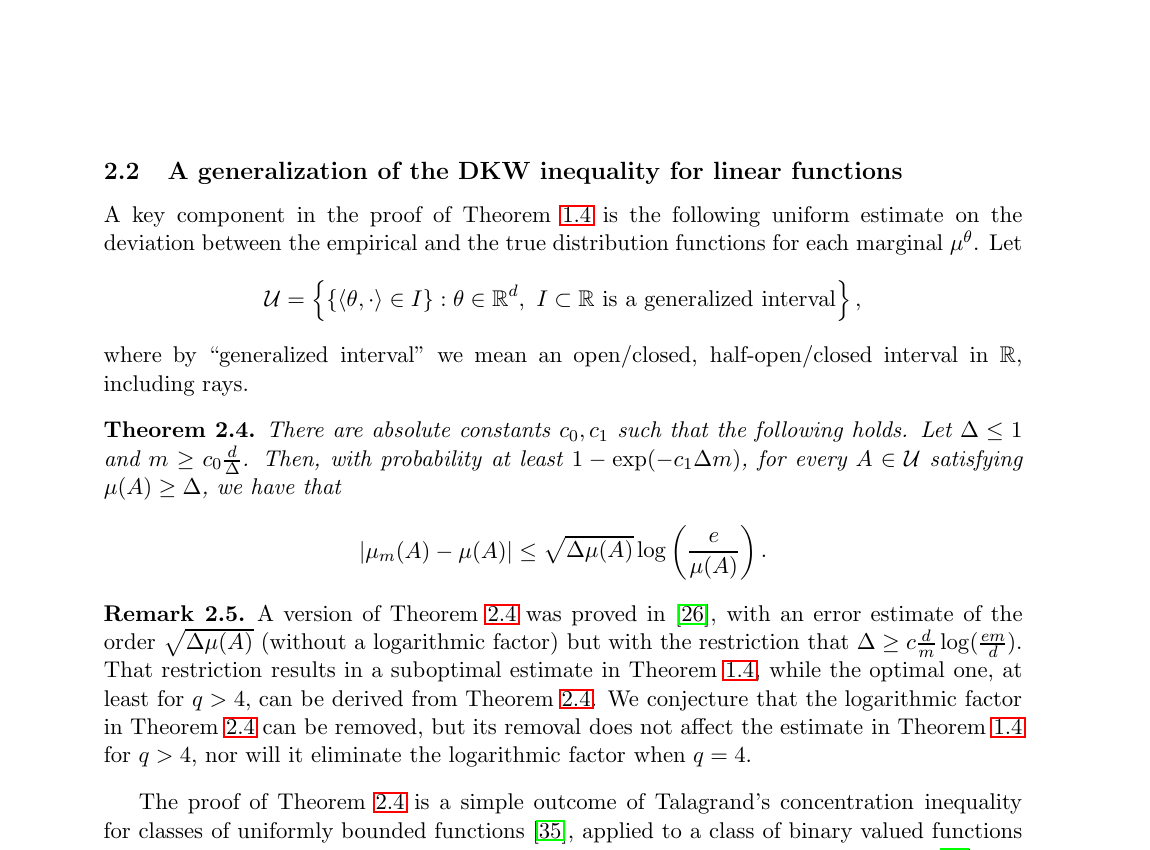
\includegraphics[width=0.92\textwidth]{figures/source_conjecture.png}
\end{center}

Here is a counterexample to that conjecture in the stated generality.

\begin{theorem}
There do not exist absolute constants $a,b,C>0$ such that, for every
probability measure $\mu$ on $\R^d$, every $0<\Delta\le1$, and every
$m\ge ad/\Delta$, one has with probability at least
$1-\exp(-b\Delta m)$ the simultaneous log-free estimate
\[
 |\mu_m(A)-\mu(A)|\le C\sqrt{\Delta\mu(A)}
 \qquad(A\in\mathcal U,\ \mu(A)\ge\Delta).
 \tag{2}
\]
The failure already occurs for centered isotropic measures on $\R^2$.
\end{theorem}

\begin{proof}
Assume that $a,b,C$ exist.  Fix a constant $\alpha>2a$ and, for every
$N\ge3$, put
\[
 v_j=\sqrt2\bigl(\cos(2\pi j/N),\sin(2\pi j/N)\bigr),
 \qquad
 \mu_N=\frac1N\sum_{j=1}^N\delta_{v_j}.
 \tag{3}
\]
The roots-of-unity identities give
$N^{-1}\sum_jv_j=0$ and
$N^{-1}\sum_jv_jv_j^{\mathsf T}=I_2$; thus $\mu_N$ is centered and
isotropic.  Moreover $|\langle v_j,\theta\rangle|\le\sqrt2$ for
$\theta\in S^1$, while isotropicity gives
$\|\langle\cdot,\theta\rangle\|_{L_2(\mu_N)}=1$.  Hence these measures also
satisfy the paper's running $L_q$--$L_2$ marginal equivalence, uniformly in
$N$ (indeed with constant $\sqrt2$ for every $q\ge2$).

Every singleton $\{v_j\}$ belongs to $\mathcal U$.  Indeed, the functional
$x\mapsto\langle v_j,x\rangle$ has a strict maximum on the support of
$\mu_N$ at $v_j$.  Choosing a ray whose endpoint lies strictly between that
maximum and the second-largest value isolates $v_j$.

Set $\Delta_N=1/N$ and $m_N=\lceil\alpha N\rceil$.  For all large $N$,
$m_N\ge 2aN=ad/\Delta_N$.  Let $K_j$ be the number of the $m_N$ samples
equal to $v_j$. Applying (2) to every singleton gives
\[
 \left|\frac{K_j}{m_N}-\frac1N\right|\le\frac CN,
 \qquad 1\le j\le N.
 \tag{4}
\]
Consequently the event in (2) is contained in
\[
 \left\{\max_{1\le j\le N}K_j\le B\right\},
 \qquad B:=\left\lceil(\alpha+1)(C+1)\right\rceil,
 \tag{5}
\]
where $B$ is independent of $N$.

We now prove that the probability in (5) tends to zero.  On one probability
space, generate an infinite sequence of independent uniform choices from
$\{1,\dots,N\}$ and an independent random variable
$L_N\sim\operatorname{Poisson}(\alpha N/2)$.  Let $Y_j$ count label $j$
among the first $L_N$ choices.  By Poisson splitting,
$Y_1,\dots,Y_N$ are independent $\operatorname{Poisson}(\alpha/2)$ random
variables.  Hence, with
\[
 q_B=\Prob\{\operatorname{Poisson}(\alpha/2)\le B\}<1,
\]
we have
\[
 \Prob\left\{\max_jY_j\le B\right\}=q_B^N\longrightarrow0.
 \tag{6}
\]
Also $\Prob\{L_N>m_N\}\to0$, for example by a standard Poisson Chernoff
bound, since $m_N$ is asymptotically twice the mean of $L_N$.
On $\{L_N\le m_N\}$ the first $L_N$ samples are contained among the first
$m_N$ samples, so $Y_j\le K_j$ for all $j$.  Therefore
\[
 \Prob\left\{\max_jK_j\le B\right\}
 \le q_B^N+\Prob\{L_N>m_N\}\longrightarrow0.
 \tag{7}
\]

In contrast, (2) asserts that its event has probability at least
\[
 1-\exp(-b\Delta_Nm_N)\longrightarrow1-\exp(-b\alpha)>0.
\]
This contradicts (5)--(7), and proves the theorem.
\end{proof}

\begin{remark}[What the example does and does not show]
The obstruction is the occupancy fluctuation of small atoms.  Thus the
logarithmic factor in (1) cannot simply be deleted for arbitrary measures,
even if centered isotropic measures are required.  The argument does not
exclude a log-free theorem under nonatomicity, a uniform density condition,
log-concavity, or another regularity assumption.  Standard maximum-load
asymptotics in fact give
$\max_jK_j\asymp\log N/\log\log N$ here, showing that some diverging loss is
unavoidable as $\Delta=1/N\downarrow0$.
\end{remark}

\paragraph{Status and search.}
This is a full negative answer to Remark~2.5 as literally stated.  The
January 2025 source revision still contains the conjecture.  Cheap run
indexes and bounded exact-title, exact-phrase, and author/topic searches found
no prior explicit resolution.  The proof is self-contained and uses no
numerical computation.

\begin{thebibliography}{9}
\bibitem{BM}
D.~Bartl and S.~Mendelson,
\emph{Structure preservation via the Wasserstein distance},
arXiv:2209.07058, current source revision January 2025.
\end{thebibliography}

\end{document}
